%Copyright 2019 Christopher M. Jermaine (cmj4@rice.edu) and Risa B. Myers (rbm2@rice.edu)
%
%Licensed under the Apache License, Version 2.0 (the "License");
%you may not use this file except in compliance with the License.
%You may obtain a copy of the License at
%
%    https://www.apache.org/licenses/LICENSE-2.0
%
%Unless required by applicable law or agreed to in writing, software
%distributed under the License is distributed on an "AS IS" BASIS,
%WITHOUT WARRANTIES OR CONDITIONS OF ANY KIND, either express or implied.
%See the License for the specific language governing permissions and
%limitations under the License.
%===============================================================
\documentclass[aspectratio=169]{beamer}
\mode<presentation> 
{
\usetheme[noshadow, minimal,numbers,riceb,nonav]{Rice}
\usefonttheme[onlymath]{serif}
\setbeamercovered{transparent}
}
\useinnertheme{rectangles}

\usepackage[english]{babel}

\usepackage{amsmath}
\usepackage{mathptmx}
\usepackage{helvet}
\usepackage{courier}
\usepackage[T1]{fontenc}
\usepackage{trajan}
\usepackage{ textcomp }
\renewcommand{\footnotesize}{\tiny}


\usepackage{listings}

\newenvironment{noindentitemize}
{ \begin{itemize}
 \setlength{\itemsep}{1.5ex}
  \setlength{\parsep}{0pt}   
  \setlength{\parskip}{0pt}
 \addtolength{\leftskip}{-2em}
 }
{ \end{itemize} }

\newenvironment{noindentitemize2}
{ \begin{itemize}
  \setlength{\itemsep}{0ex}
  \setlength{\parskip}{0pt}
  \setlength{\parsep}{0pt}   
  \addtolength{\leftskip}{-2em}  }
{ \end{itemize} }

\lstnewenvironment{SQL}
  {\lstset{
        aboveskip=5pt,
        belowskip=5pt,
        escapechar=!,
        mathescape=true,
        upquote=true,
        language=C,
        basicstyle=\linespread{0.94}\ttfamily\footnotesize,
        deletekeywords={VALUE, PRIOR},
        showstringspaces=true}
        \vspace{0pt}%
        \noindent\minipage{0.47\textwidth}}
  {\endminipage\vspace{0pt}}
  
\newcommand{\LIKES}{\textrm{LIKES}} 
\newcommand{\FREQUENTS}{\textrm{FREQUENTS}} 
\newcommand{\SERVES}{\textrm{SERVES}} 
\newcommand{\CAFE}{\textrm{CAFE}} 
\newcommand{\COFFEE}{\textrm{COFFEE}} 
\newcommand{\DRINKER}{\textrm{DRINKER}} 
\newcommand{\ALLPEEPS}{\textrm{ALLPEEPS}} 
\newcommand{\ALLCOMBOS}{\textrm{ALLCOMBOS}} 

\setbeamerfont{block body}{size=\tiny}

%===============================================================%

\title[]
{Tools \& Models for Data Science}

\subtitle{Deep Neural Networks (4): LSTM}

\author[]{Chris Jermaine \& Risa Myers}
\institute
{
  Rice University 
}

\date[]{}

\subject{Beamer}

\begin{document}

\begin{frame}
 \titlepage
\end{frame}
%***********************************************************
\begin{frame}{RNN}

\begin{itemize}
	\item Have a chain of repeating ``modules'' 
	\begin{itemize}
	\item Each is a simple feed-forward network
	\item Often a single, fully-connected layer
	\item Each neuron uses some standard activation function (tanh, logistic)
	\end{itemize}
\end{itemize}
\end{frame}
%***********************************************************
\begin{frame}{Unrolling RNNs}

\begin{itemize}
	\item Training/prediction works via unrolling
	\item Input at each time tick concatenated with last internal state
\begin{itemize}
	\item Sent through a tanh/logistic layer
	\item Result of that layer used to produce output, sent into next tick (Jordan network)
	\item Each module is 1 iteration of the network
\end{itemize}
\end{itemize}
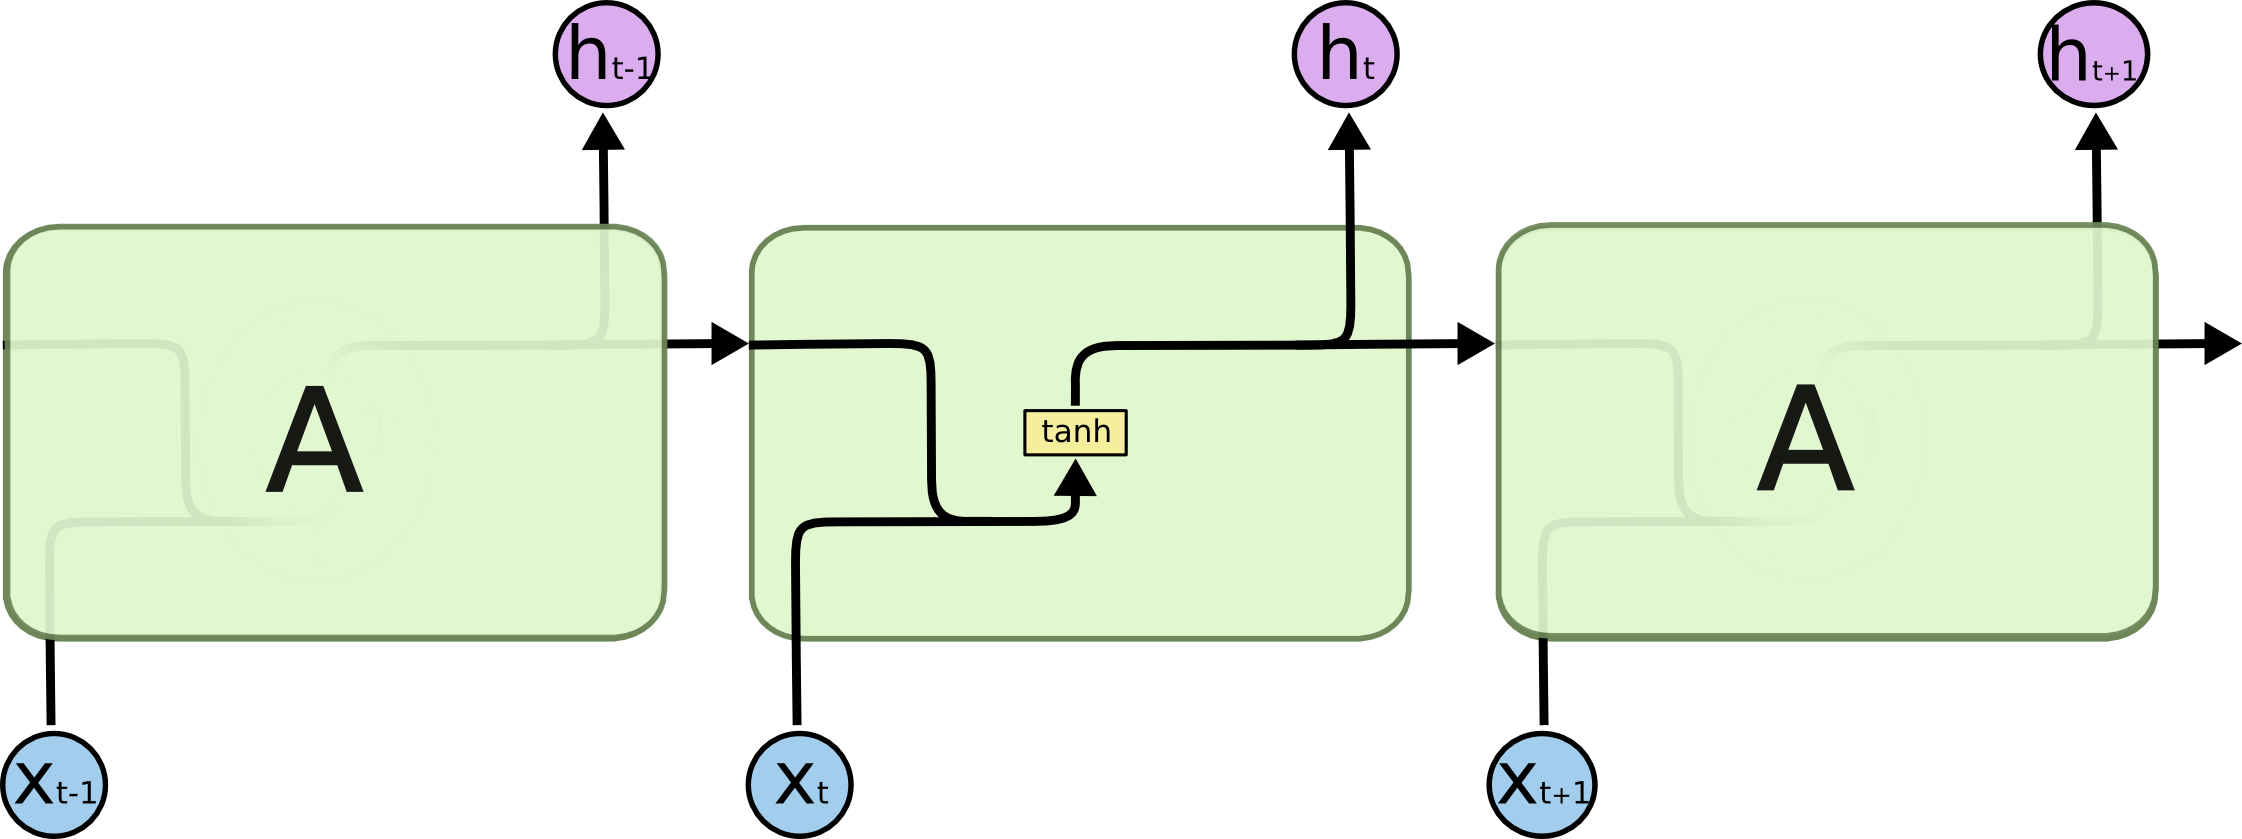
\includegraphics[width=0.8\textwidth]{lectLSTM/LSTM3-SimpleRNN.png}
\footnote{Reprinted with permission. \url{http://colah.github.io/posts/2015-08-Understanding-LSTMs/}}
\end{frame}
%***********************************************************
\begin{frame}{Problem With RNNs}

\begin{itemize}
	\item The ``vanishing gradient'' problem
	\item During back-propagation
	\begin{itemize}
	\item Update magnitude drops exponentially with distance from output
	\item Recall 
        $$ \frac{\partial L}{\partial w_{i,j,k}} = \frac{\partial L}{\partial y_{i,k}}
                                                \frac{\partial y_{i,k}}{\partial v_{i,k}}
                                                \frac{\partial v_{i,k}}{\partial w_{i,j,k}}$$
	\item If activation function is logistic function $\sigma$ then
	$\frac{\partial y_{i,k}}{\partial v_{i,k}} = \sigma (v_{i,k})(1 - \sigma (v_{i,k}))$
	\item Means you have a multiplier that maxes out at 0.25
	\item Max value is when $v_{i,k} = 0.5$
	\item $\sigma(0.5) = 0.25$
	\item As you back-propagate, you keep multiplying by this in DP... $.25 \times .25 \times .25 ...$ gradient gets tiny
	\end{itemize}
	\item Result is that output at time tick $t$...
	\begin{itemize}
	\item ...has little interaction with input at tick $t - 100$ during back-propagation
	\item Practically speaking: means back-propagation has limited-duration memory
	\end{itemize}
\end{itemize}
\end{frame}
%***********************************************************
\begin{frame}{LSTM}

\begin{itemize}
	\item First proposed in 1997 by Hichreiter/Schimiduber
	\begin{itemize}
	\item Uses a more complicated architecture in each recurrent unit
	\item Now used in most state-of-the-art sequence-based ML
	\item Translation, text processing, speech-to-text, many others...
	\end{itemize}
\end{itemize}
\end{frame}
%***********************************************************
\begin{frame}{No Vanishing Gradients?}
        \begin{itemize}
	\item Key idea: have a state that passes from tick to tick
	\begin{itemize}
	\item Explicitly decide which part of state to update
	\item Which part of the state to forget
	\item And which part of the state affects the output
	\end{itemize}
	\item If ``forget'' is turned off 
	\begin{itemize}
	\item State just passes through un-modified
	\item Derivative of identity function is 1
	\item So gradient updates during back-propagation pass through un-modified
	\item No vanishing gradients!
	\end{itemize}
\end{itemize}
\end{frame}
%***********************************************************
\begin{frame}{Basic LSTM Architecture}
\begin{itemize}
	\item An LSTM-based RNN is unrolled into a sequence of LSTM ``modules''
	\begin{itemize}
	\item Each module accepts input at a particular time tick
	\item As well as state (``long term'' memory) and last output (``short term'' memory)
	\item Uses those to output a view of its current state	
	\end{itemize}
\end{itemize}
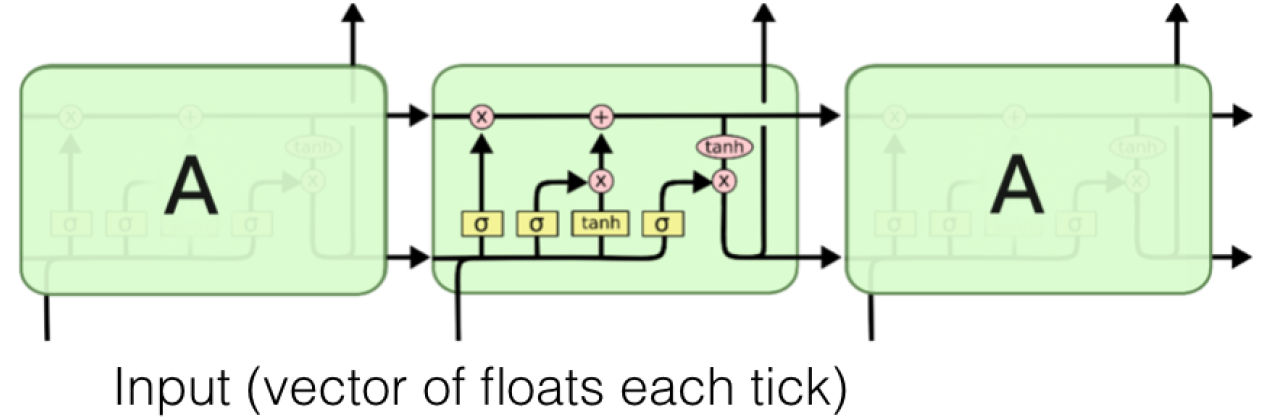
\includegraphics[width=0.8\textwidth]{lectLSTM/LSTMNew.png}
\footnote{Reprinted with permission. \url{http://colah.github.io/posts/2015-08-Understanding-LSTMs/}}

\end{frame}
%***********************************************************
\begin{frame}{A Note on Notation}
\begin{itemize}
	\item In this pic:
	\begin{itemize}
	\item Vectors travel along lines
	\item A circle/oval represents application of a function to each dimension in a vector
	\item A rectangle represents a neural network
	\item $\sigma$ means a logistic activation layer at the top
	\item tanh means a hyperbolic tangent activation layer at the top
	\end{itemize}
\end{itemize}
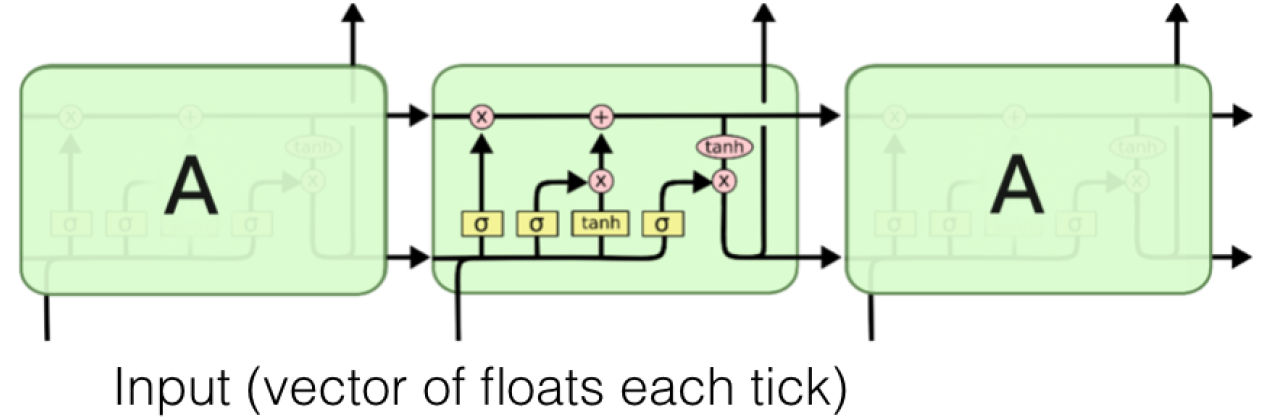
\includegraphics[width=0.8\textwidth]{lectLSTM/LSTMNew.png}
\footnote{Reprinted with permission. \url{http://colah.github.io/posts/2015-08-Understanding-LSTMs/}}
\end{frame}
%***********************************************************
\begin{frame}{Now, Let's Go Over the Parts in Detail}

\begin{columns}
\begin{column}{0.5\textwidth}
        \begin{itemize}
	\item At the top is a state (long term memory) that passes through the unit
	\begin{itemize}
	\item Possibly unimpeded
	\item Possibly modified
	\end{itemize}
\end{itemize}
\end{column}
\begin{column}{0.5\textwidth}
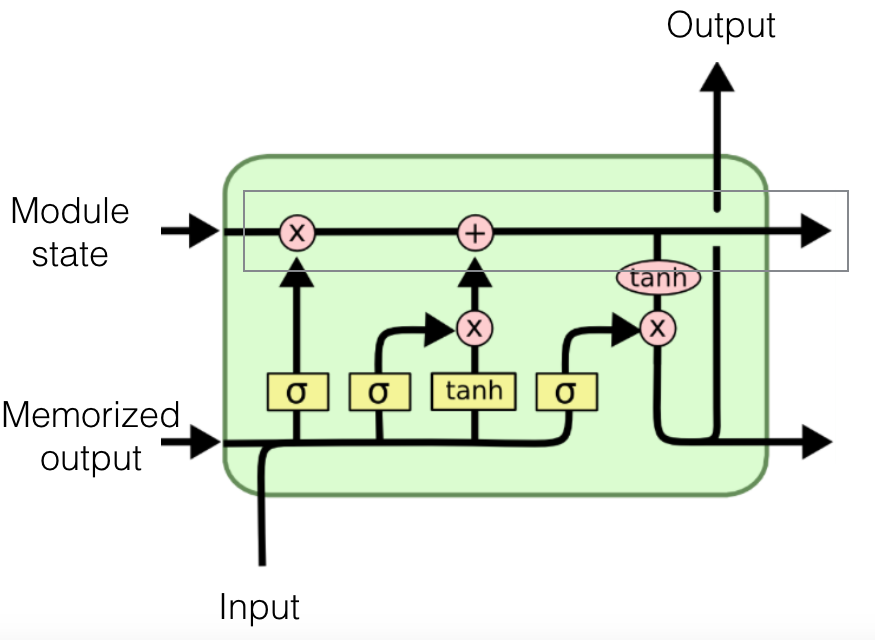
\includegraphics[width=1\textwidth]{lectLSTM/highway.png}
\footnote{Reprinted with permission.\\ \hspace{1.7em}\url{http://colah.github.io/posts/2015-08-Understanding-LSTMs/}}
\end{column}
\end{columns}
\end{frame}
%***********************************************************
\begin{frame}{Changing Long-Term Memory Contents}

\begin{columns}
\begin{column}{0.6\textwidth}
\begin{itemize}
	\item There are two operations that can affect the state...
	\begin{itemize}
	\item An item-by-item vector multiplication
	\item Known as the ``forget gate''
	\item And an item-by-item vector addition
	\item Known as the ``input gate''
	\end{itemize}
\end{itemize}
\end{column}
\begin{column}{0.4\textwidth}
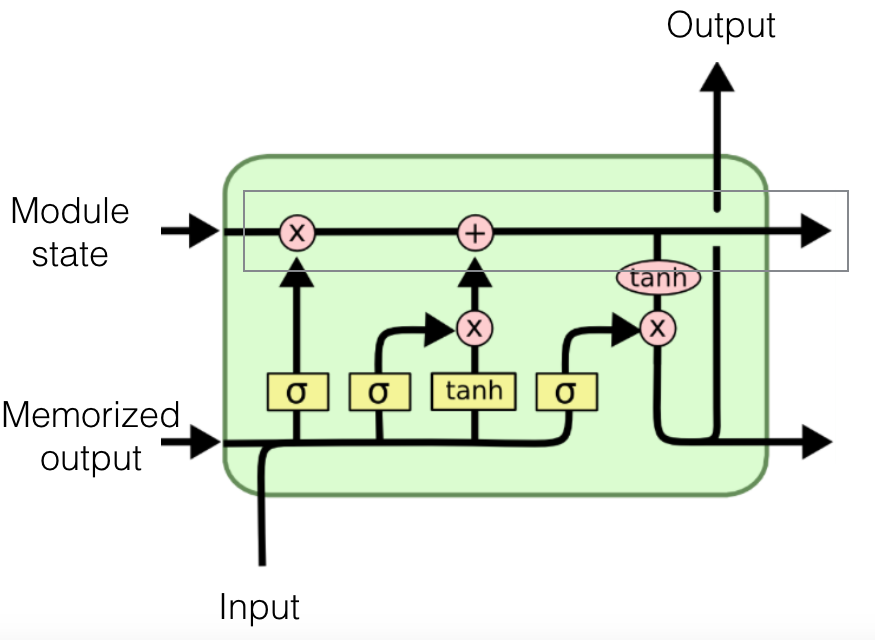
\includegraphics[width=1\textwidth]{lectLSTM/highway.png}
\footnote{Reprinted with permission.\\ \hspace{1.7em}\url{http://colah.github.io/posts/2015-08-Understanding-LSTMs/}}
\end{column}
\end{columns}
\end{frame}
%***********************************************************
\begin{frame}{At the Bottom...}

\begin{columns}
\begin{column}{0.5\textwidth}
\begin{itemize}
	\item Memorized output and new input flow though the unit
        \begin{itemize}
        \item They control the forget gate and the input gate
        \item Might see new input and decide not to modify state
        \item Or might decide to throw out old state and rebuild
        \end{itemize}
	\item At the end...
	\begin{itemize}
	\item Input and state of memory used to produce output
	\end{itemize}
\end{itemize}
\end{column}
\begin{column}{0.5\textwidth}
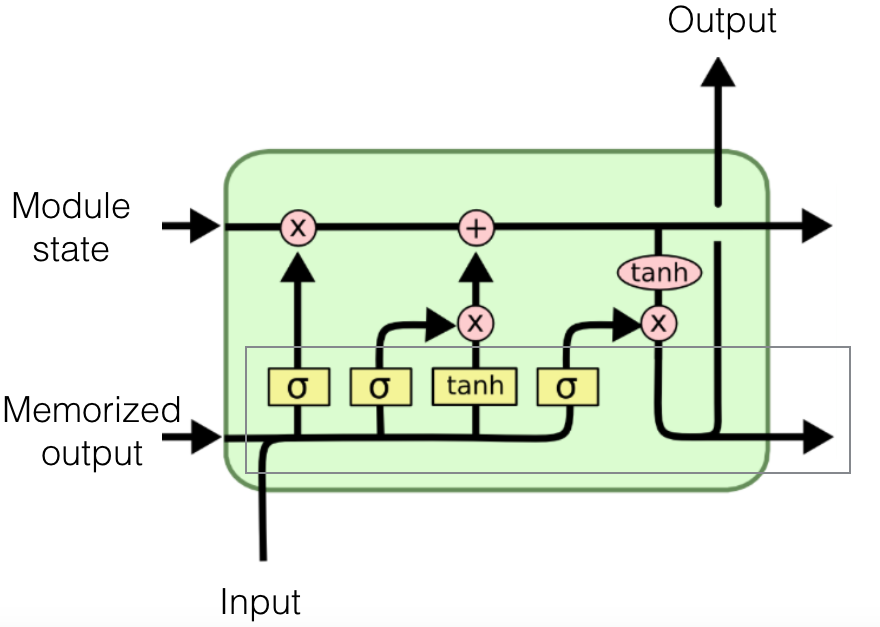
\includegraphics[width=1\textwidth]{lectLSTM/memorized.png}
\footnote{Reprinted with permission.\\ \hspace{1.7em}\url{http://colah.github.io/posts/2015-08-Understanding-LSTMs/}}
\end{column}
\end{columns}
\end{frame}
%***********************************************************
\begin{frame}{Now Let's Walk Through Input Processing}

\begin{columns}
\begin{column}{0.5\textwidth}
\begin{itemize}
	\item First we run the ``forget gate''
	\begin{itemize}
		\item Last output and new input pass through a NN
		\item With a logistic layer at top
		\item Produces all values from 0 to 1
		\item Item-by-item multiply with state
	\end{itemize}
\end{itemize}
\end{column}
\begin{column}{0.5\textwidth}
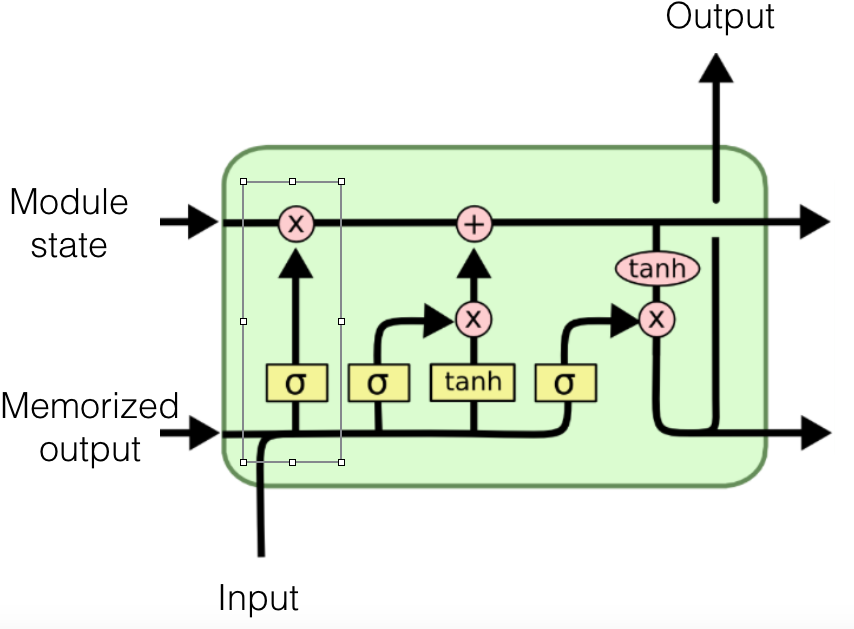
\includegraphics[width=1\textwidth]{lectLSTM/dampen.png}
\footnote{Reprinted with permission.\\ \hspace{1.7em}\url{http://colah.github.io/posts/2015-08-Understanding-LSTMs/}}
\end{column}
\end{columns}
\end{frame}
%***********************************************************
\begin{frame}{Forget Gate}

\begin{columns}
\begin{column}{0.5\textwidth}
\begin{itemize}
	\item Controls what items in state are forgotten
	\begin{itemize}
		\item Logistic produces a 0 for a dimension?
		\item Then you will zero-out that dimension in the input
	\end{itemize}
\end{itemize}
\end{column}
\begin{column}{0.5\textwidth}
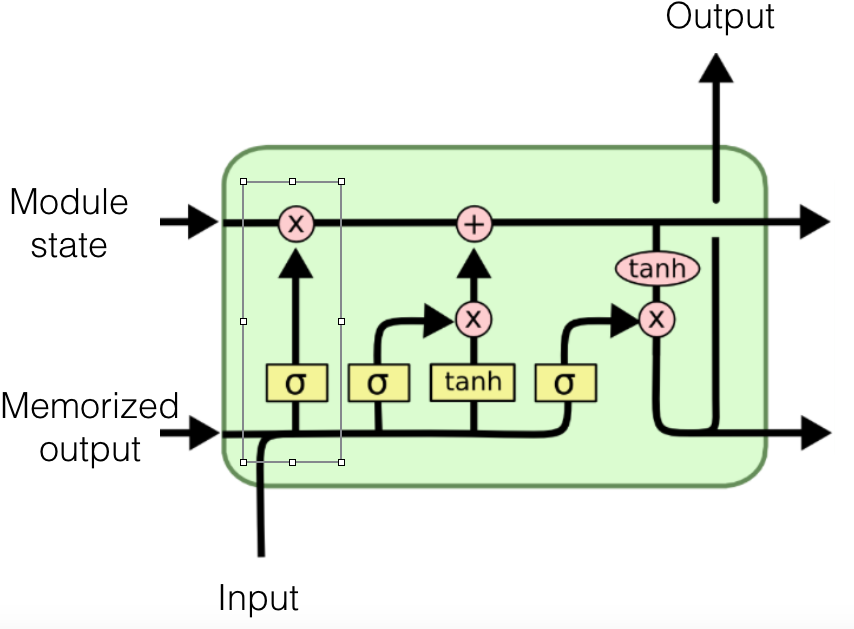
\includegraphics[width=1\textwidth]{lectLSTM/dampen.png}
\footnote{Reprinted with permission.\\ \hspace{1.7em}\url{http://colah.github.io/posts/2015-08-Understanding-LSTMs/}}
\end{column}
\end{columns}
\end{frame}
%***********************************************************
\begin{frame}{Next Is the ``Input Gate''}

\begin{columns}
\begin{column}{0.5\textwidth}
\begin{itemize}
	\item Input plus last output passes through two NNs
	\begin{itemize}
		\item One with a tanh layer at the top...
		produces activations from -1 to +1
		\item One with a logistic layer at the top...
		produces activations from 0 to 1
	\end{itemize}
	\item Item-by-item multiply produces a vector of updates to state
	\begin{itemize}
		\item This update is added into the long term memory
		\item This is the ``input gate''
	\end{itemize}
\end{itemize}
\end{column}
\begin{column}{0.5\textwidth}
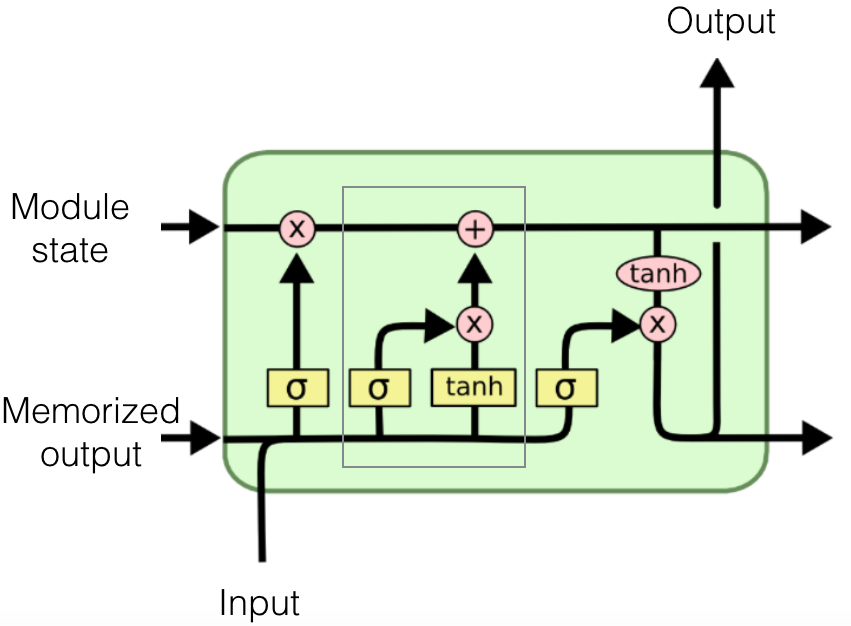
\includegraphics[width=1\textwidth]{lectLSTM/adding.png}
\footnote{Reprinted with permission.\\ \hspace{1.7em}\url{http://colah.github.io/posts/2015-08-Understanding-LSTMs/}}
\end{column}
\end{columns}
\end{frame}
%***********************************************************
\begin{frame}{Producing Output}

\begin{columns}
\begin{column}{0.5\textwidth}
\begin{itemize}
	\item Now we have modified the state (long-term memory)
	\item Use the state to produce the output
	\begin{itemize}
		\item First, push state through a tanh layer
		\item Maps memory to values from -1 to +1
	\end{itemize}
\end{itemize}
\end{column}
\begin{column}{0.5\textwidth}
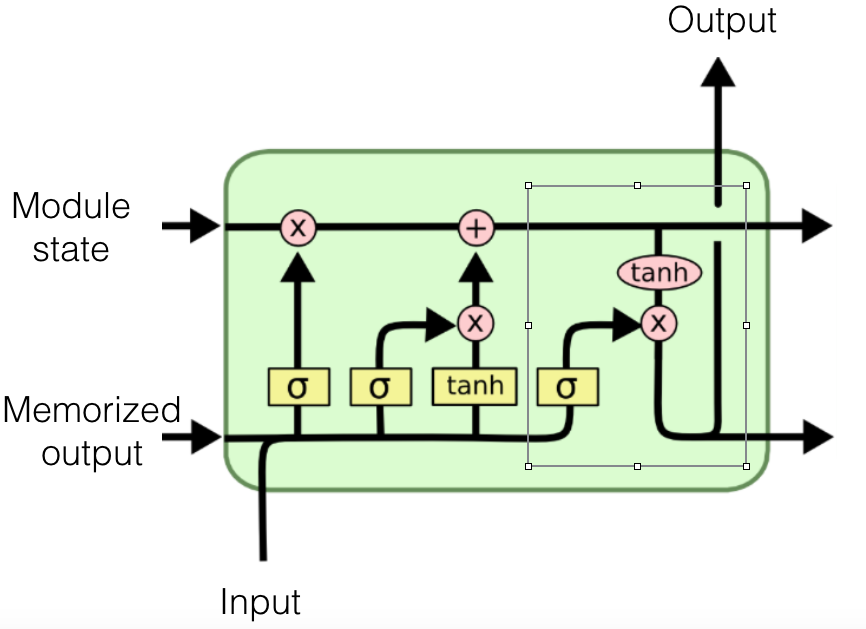
\includegraphics[width=1\textwidth]{lectLSTM/output.png}
\footnote{Reprinted with permission.\\ \hspace{1.7em}\url{http://colah.github.io/posts/2015-08-Understanding-LSTMs/}}
\end{column}
\end{columns}
\end{frame}
%***********************************************************
\begin{frame}{Output Gate}

\begin{columns}
\begin{column}{0.5\textwidth}
\begin{itemize}
	\item And push the input and last output through a final NN
	\begin{itemize}
		\item With a logistic activation at top
		\item Produces values between 0 and 1
		\item Item-by-item multiply with post-processed state
		\item This decides what part of the state to output
		\item Called the ``output gate''
	\end{itemize}
\end{itemize}
\end{column}
\begin{column}{0.5\textwidth}
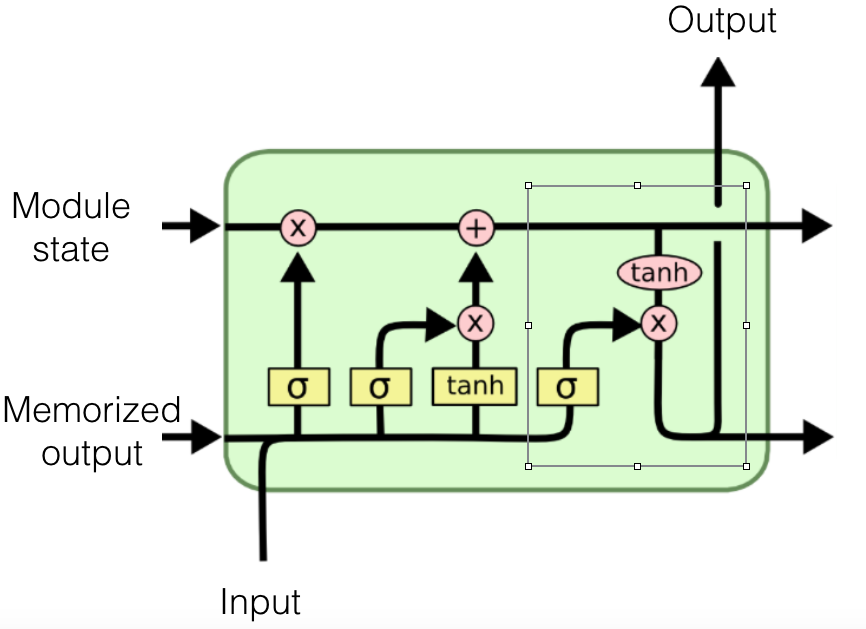
\includegraphics[width=1\textwidth]{lectLSTM/output.png}
\footnote{Reprinted with permission.\\ \hspace{1.7em}\url{http://colah.github.io/posts/2015-08-Understanding-LSTMs/}}
\end{column}
\end{columns}
\end{frame}
%***********************************************************
\begin{frame}{Output Typically Pushed Through a Final NN}

\begin{itemize}
	\item Output is simply a subset of the long-term memory
	\begin{itemize}
		\item Like a brain dump
		\item Simply reports encoded contents of the memory
		\item Not directly useful to solve any task
		\item Need to post-process (decode) it
	\end{itemize}
        \item For example, if task is part-of-speech (POS) tagging
        \begin{itemize}
                \item We might push output through a NN
		\item Topped with a tanh layer
		\item One neuron for each POS (noun, verb, adjective, etc.)
                \item Push neuron outputs through a softmax
		\item Output of softmax chooses final POS
        \end{itemize}
\end{itemize}
\end{frame}
%***********************************************************
\begin{frame}{Stacking These Modules}

\begin{itemize}
	\item Say we want some more learning capacity
	\begin{itemize}
                \item Can ``stack'' LSTMs
	\end{itemize}
	\item At each time tick
	\begin{itemize}
		\item Have $m$ stacked LSTM modules
		\item Creates a stack with $m$ layers
		\item Each with its own set of parameters
		\item LSTM in layer $l$ has same internal NN params, no matter the time tick
	\end{itemize}
\end{itemize}
\end{frame}
%***********************************************************
\begin{frame}{Stacking LSTMs}

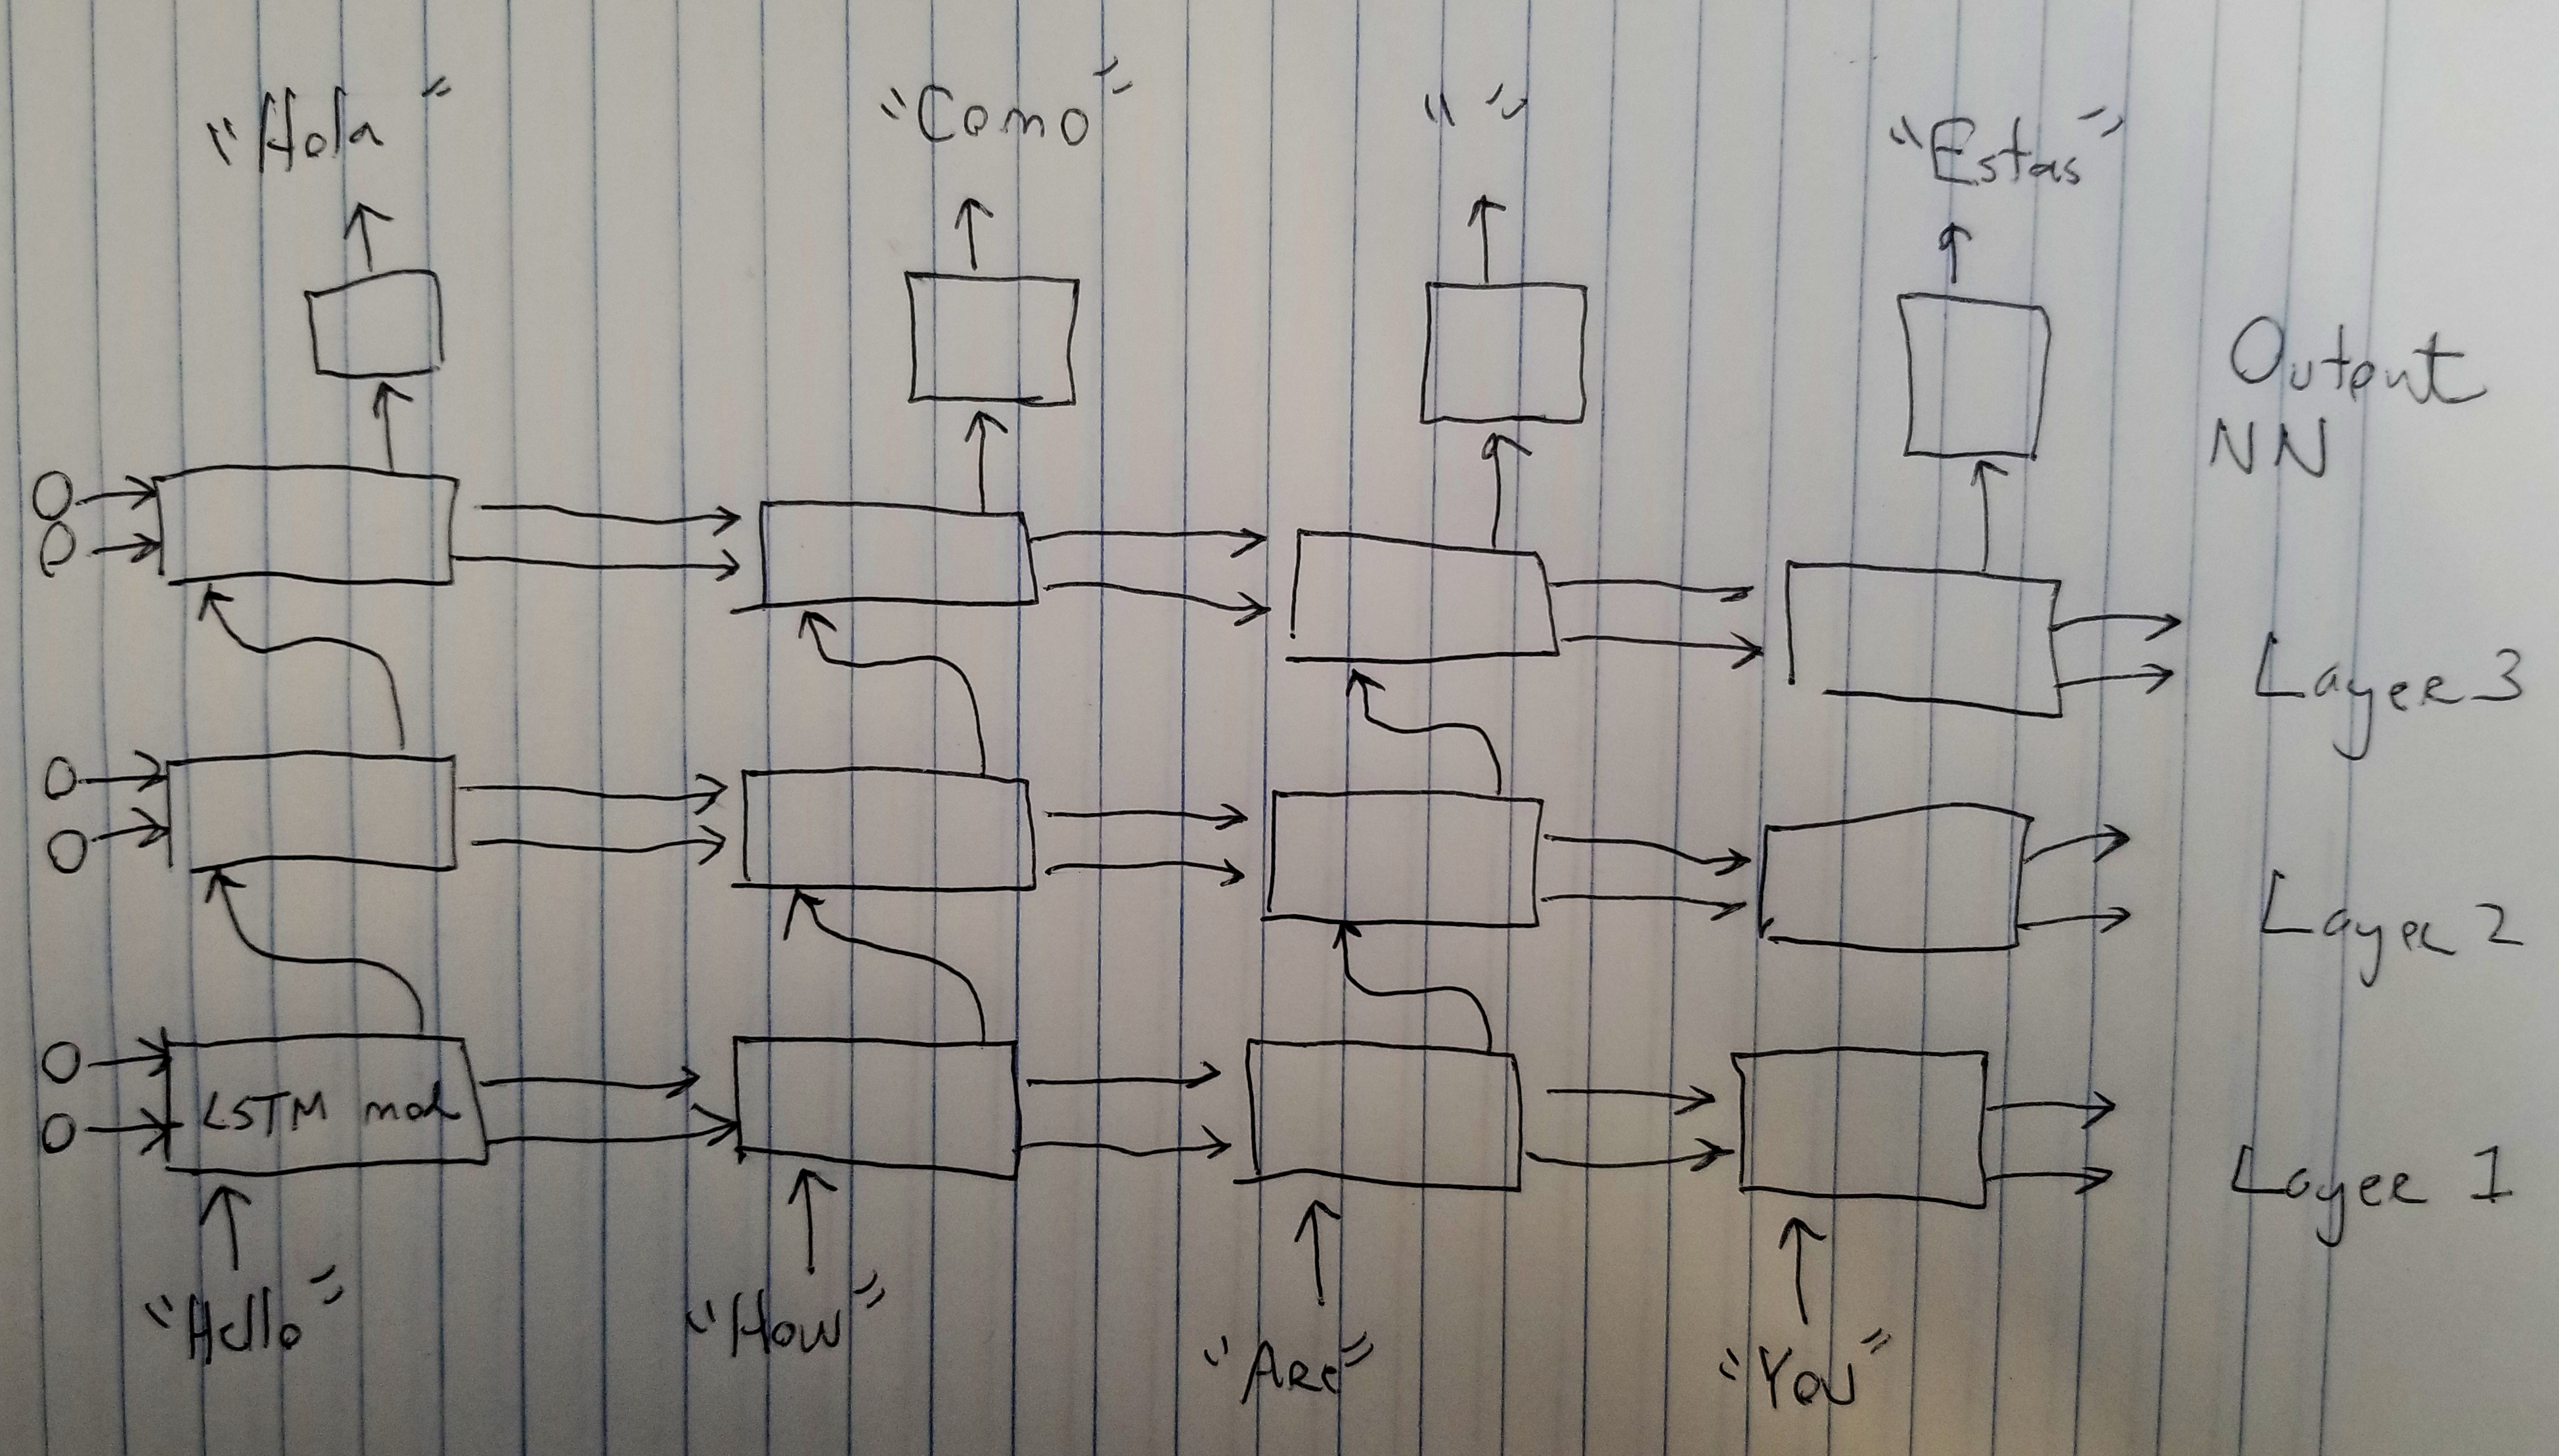
\includegraphics[width=0.9\textwidth]{lectLSTM/Stacked.jpg}
\end{frame}
%***********************************************************
\begin{frame}{Creates a Grid of LSTMs}
\begin{itemize}
	\item LSTM layer $l$ at time tick $t$
	\begin{itemize}
		\item Sends its state and output to LSTM module at layer $l$, time tick $t + 1$
		\item Sends its output to LSTM module at layer $l + 1$, time tick $t$
	\end{itemize}
	\item LSTM layer $1$ at time tick $t$
	\begin{itemize}
		\item Gets its input externally, from input stream
		\item All other layers get their input from previous layer at tick $t$
	\end{itemize}
	\item The output from the last/top layer at tick $t$...
	\begin{itemize}
		\item Is used to produce output at tick $t$
	\end{itemize}
\end{itemize}
\end{frame}
%***********************************************************
\begin{frame}{Uses for Stacked LSTM Modules}

\begin{itemize}
%https://machinelearningmastery.com/stacked-long-short-term-memory-networks/
	\item Recognize more complex concepts/objects % lines to shapes to objects
	\item Learn hierarchies
	\item Predict activity from multiple signals
\end{itemize}
\end{frame}
%***********************************************************

\begin{frame}{Questions?}
\end{frame}
\end{document}
